\section{Plugins}
\label{sec:plugins}

There are three types of plugins: \textit{Effectors}, \textit{Perceivers}, and \textit{Utility}. Their responsibility is to propose actions, to receive external world stimuli and support its peers, respectively. For the developers, the \textit{Effectors} are the only ones capable of proposing actions and changing the status of other plugins, the remaining types are identical, only differing by its name.

Furthermore, one of the goals of this project is to provide the developers with the flexibility to reuse their components on different scenarios with little to no additional effort. For this purpose, researchers only need to focus on the essentials components of the plugin as the system already provides the tools to handle, for example, optional \ac{GUI} and, more importantly, configuration files to change the rapport \textit{Effectors}' parameters specified throughout Chapter~\ref{chap:rapportModel}. The configuration file is a \ac{XML} document that is loaded during the plugin's initialisation, and can be modified afterwards (and saved) in runtime by accessing the configuration file (Listing~\ref{lst:facialExpressionsSettings} in Appendix B) by clicking on the settings icon depicted on each row in Figure~\ref{fig:pluginList}. The major advantage is that the developer does not need to recompile the plugins just to make this change. Lastly, the plugin's \ac{GUI} can be opened from the controller's user interface (Figure~\ref{fig:pluginList}). An \textit{Effector} that mimics facial expression is listed in Listing~\ref{lst:facialExpressionsSourceCode} in Appendix C.

\subsection{Effector}
\label{sub:sec:effectorPlugin}

%One could argue that another \textit{Effector} could lock the Face Action Group with an empty action with higher priority, however, this is an elaborate solution that adds unnecessary complexity to the system. An easier solution is to, track the current gaze target, and deactivate and enable the \textit{Effectors} that rely on direct eye contact.

The main task of the \textit{Effectors} was described previously in Section~\ref{sub:sec:managingActions}. However, during development, we identified a key use case that greatly impacts interactions. During the development of the scenario described in Chapter~\ref{chap:userstudies}, we identified that it would be helpful if we could deactivate and enable plugins in runtime, allowing specific rapport strategies to only affect discrete sections of the scenario. For example, deactivate idle behaviour if the agent is attentive to the task. This mechanism should be handled by a separate higher-level plugin that maps the agent's state to the list of enabled rapport strategies, leaving the essential to the \textit{Effector}.

Another key issue that emerged was internal conflict within the \textit{Effector} where it would interrupt himself repeatedly. For example, during the initial stages, the behavioural mimicry rapport \textit{Effectors} from the rapport model, described in Section~\ref{sub:model_Coordination}, were interrupting themselves regularly because the \textit{Perceiver} was continuously notifying them. To solve this issue, we added, transparently to the developer, a mechanism to track internally the proposed actions, and an additional parameter that specifies the minimum interval of time between action proposals. The researcher can choose on of the following levels:

\begin{itemize}
	\item \textbf{Unrestricted}: the \textit{Effector} must explicitly manage its proposed actions;
	\item \textbf{One Action Globally}: the \textit{Effector} cannot interrupt itself unless with a proposal with higher priority;
	\item \textbf{One Action Per Group}: same as \textit{One Action Globally} but granulated to the \textit{Group}.
\end{itemize}

In short, the task greatly influences how the different plugins will have to cooperate with one another in order to satisfy the behavioural goals of the interaction. For example, it is crucial to properly define the priority of the action proposals as it is fundamental to manage which actions will be triggered and which actions will be interrupted at any given time. To recall the reader, behaviours triggered by singular events should have higher priorities than events that happen commonly. For example, a surprise emotion (an emotion typically raised by an unexpected sudden event) should have higher priority than, for example, a happy facial expression that is at the moment mimicking the interactional partner emotion.

\subsection{Agent Actions Manager}
\label{sub:sec:agentActionsManager}

%Mencionar que é este o plugin que tem a Thalamus Connection para executar acções

Agent Actions Manager is a \textit{Utility} plugin with the following goals:
\begin{itemize}
	\item Monitors agent's actions to notify the \textit{Rapport Controller};
	\item Provide convenient wrappers for common action proposals, describing both execution and interruption descriptions ($E$ and $I$): animations, utterances, vocalisations, sounds, head nods, head shakes, and gaze;
	\item Provide non-technical researchers with the tools to change the agent's behaviour given the dyadic state of the interaction, without worrying about implementation details.
\end{itemize}

The first objective is achieved by monitoring the messages that both \textit{Speech Server} and \textit{Nutty Tracks} send to the \textit{Thalamus Network}, and compare the actions' identifiers with the stored ones. They both notify whenever their actions have started or have finished, therefore this plugin just monitors those messages containing the action \texttt{id} and redirects them to the \textit{Rapport Controller}. The second objective aims to reduce the amount of code required to specify common action proposals. Therefore, the \textit{Effectors}, in order to use the provided tools, have to request the \textit{Rapport Controller}, the Agent Actions Manager \textit{Utility} plugin during the \textit{Initialise dependencies} stage of the initialisation (Figure~\ref{fig:pluginLifecycle} in Section~\ref{sub:sec:pluginLifecycle}).

\begin{figure}[H]
	\centering
	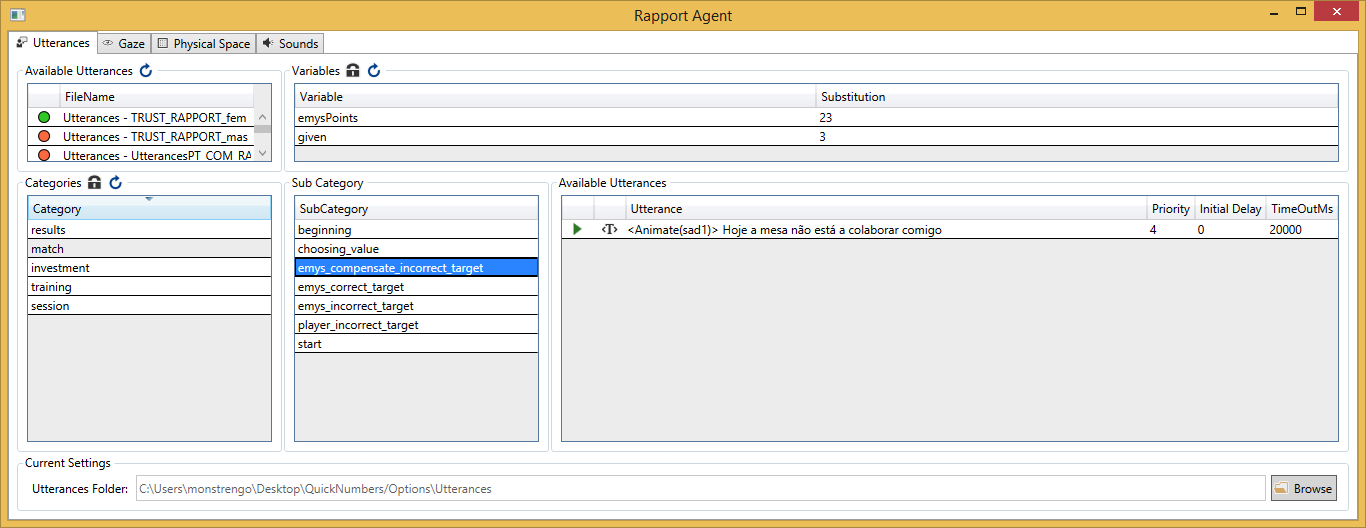
\includegraphics[width=\textwidth]{images/ScreenshotAgentsManager.png}
	\caption{\ac{GUI} representation of the Agent Action Manager \textit{Utility} plugin.}
	\label{fig:agentActionsManagerScreenshot}
\end{figure}

To accomplish the last goal, the Agent Actions Manager \textit{Utility} plugin, similar to \textit{Skene}, provides a \ac{GUI} that provides non-technical researchers with the tools to collaboratively change the agent's behavioural rules or utterances (Figure~\ref{fig:agentActionsManagerScreenshot}). However, these utterances take advantage of the prioritisation mechanism defined in the rapport model in Chapter~\ref{chap:rapportModel}. For this purpose, following Expression~\ref{eq:behaviour} and Table~\ref{fig:extended:utterances}, researchers can provide the following optional parameters: priority, delay, and timeout. These parameters will default to, the utterance priority, 0 and the utterance's timeout, respectively. 

\begin{equation}
	<action(arg_1, arg_2, ..., arg_n, [priority], [delay], [timeout])>
	\label{eq:behaviour}
\end{equation}

Similar to \textit{Skene}, the set of utterances can be imported from a \ac{CSV} file (using the format specified in Appendix D) and edited directly in the \ac{GUI}. Moreover, the developer may specify substitution variables by adding $|Variable|$ to the content of the utterance. The values of these substitution variables can be defined in the \ac{GUI} or in runtime by the \textit{Effectors}. If there are multiple variables with the same identifier, the ones provided by the \textit{Effector} will override the ones specified in the \ac{GUI}. Lastly, if there are multiple utterances for the same category and subcategory, only one is selected randomly as long as it was not selected in the past.

\begin{table}[H]
	\centering
	\begin{tabular}{|l|l|l|l|l|l|}
	\hline
	\multicolumn{1}{|c|}{\textbf{Category}} & \multicolumn{1}{c|}{\textbf{Subcategory}} & \textbf{Utterance}                                                                                      & \textbf{Priority} & \textbf{Delay (ms)} & \textbf{Timeout (ms)} \\ \hline	
	intro & greet & \specialcell{Hi $|$\textit{Name}$|$!$<$gaze(person)$>$} & 2 & 0 & 30000 \\ \hline
	game & score & \specialcell{Yey!$<$Animate(surprise2,3)$>$} & 2 & 0 & 30000 \\ \hline
	game & results & \specialcell{Managed $|$\texttt{Points}$|$!\\$<$gaze(person,3,500,5000)$>$} & 2 & 0 & 30000 \\ \hline
	end & ending & \specialcell{Thank you for your participation!\\$<$animate(happy4,4,1000)$>$} & 3 & 0 & 30000 \\ \hline		
	\end{tabular}
	\caption{Set of utterances compatible with the framework. Set of utterances compatible with \acf{SERA}. Actions are delimited by $<$ and $>$, and substitution variables by $|$.}
	\label{fig:extended:utterances}
\end{table}




%The \ac{GUI} (Figure~\ref{fig:agentActionsManagerScreenshot}) was done from scratch as the \textit{Rapport Controller} uses a more recent technology, \ac{WPF}.